\LaTeX はL. Lamportの開発した文書清書ソフトウェアである。もともとは、D. Knuthの開発した \TeX と呼ばれるソフトウェアで、これを使いやすく拡張したものである。近年では、数式関連の機能をさらに拡張したAMS\LaTeX も広く使われている。\LaTeX はワードプロセッサのようなソフトウェアではない。画面を見ながら文書を整形しその見たままの姿が印刷結果となるのがワードプロセッサである。例えば代表的なワードプロセッサであるMicrosoft Office Wordでは、段落や2段組、箇条書などの編集を画面を見ながら行えて、そして画面のイメージがほぼそのまま印刷される。一方、\LaTeX では見たままが印刷結果となるわけではないが、ワードプロセッサに匹敵する強力な清書機能を持っている。とくに、\LaTeX は数式の清書能力に長けている。

\section{\LaTeX の実行}
\label{sec:latex:intro}

では、さっそく例を見てみよう。適当なエディタで
\begin{reidai}
\label{reidai:latex:ex}
\begin{verbatim}
\documentclass{jarticle}
\begin{document}
$a$のまわりのテイラー展開
\begin{equation}
f(x) = \sum_{n=0}^{\infty} \frac{f^{(n)}(a)}{n!}(x-a)^n
\end{equation}
\end{document}
\end{verbatim}
\end{reidai} \noindent
と入力してみよう。このファイルを \texttt{ex.tex} という名前で保存する。このファイルを \LaTeX で処理するには、\texttt{platex}コマンド\footnote{日本語版\LaTeX 。英語のみを含む文書を処理する場合には、\texttt{latex}コマンドを使えばよい。}と\texttt{dvipdfmx}コマンドを実行する。
\begin{commandline2}
\prompt \underline{platex ex.tex}\\
\prompt \underline{dvipdfmx ex.dvi}
\end{commandline2} \noindent
一行目の \texttt{platex}コマンドでDVIファイル(\texttt{ex.dvi})が生成される。DVIは{\textbf{d}e\textbf{v}ice-\textbf{i}ndependent file format}の略で、最終的な出力形式(今の例ではPDF)に依存しない出力形式である。\texttt{dvipdfmx}コマンドは、このDVIファイルからPDF形式のファイルを生成する。これらのコマンドの実行後、\texttt{ex.pdf}というファイルができていれば成功である。では処理結果を見てみよう。Mac OS Xで作業している場合には、
\begin{commandline2}
\prompt \underline{open ex.pdf}
\end{commandline2} \noindent
Linuxで作業している場合には、
\begin{commandline2}
\prompt \underline{evince ex.pdf}
\end{commandline2} \noindent
でPDFファイルを開くことができる。結果は以下のようになっているはずである。
\renewcommand{\theequation}{1}
\begin{kekka}
\label{kekka:ex}
$a$のまわりのテイラー展開
\begin{equation}
 f(x) = \sum_{n=0}^{\infty} \frac{f^{(n)}(a)}{n!}(x-a)^n
\end{equation}
\vspace{0pt}
\end{kekka}

\paragraph{この章のまとめ}

\begin{itemize}
\item \LaTeX ファイルの拡張子は\texttt{.tex}である。
\item \LaTeX を使うには、\verb|platex| コマンドを実行する。
\item \texttt{platex}コマンドを実行すると、DVIファイル(拡張子は \texttt{.dvi})が生成される。
\item DVIファイルをPDF形式に変換するには、\verb|dvipdfmx| コマンドを実行する。
\item PDFファイルを見るには、``\verb|open PDFファイル名|'' (iMacの場合)、あるいは``\verb|evince PDFファイル名|'' (Linuxの場合)を実行する。
\end{itemize}

\section{\LaTeX に関する全体的なこと}
\label{sec:latex:global}

すでに例\ref{reidai:latex:ex}で見たとおり、\LaTeX のソースファイルには、本文以外の情報も書き込まれている。具体的には、
\begin{reidai}
\label{reidai:latex:template}
\begin{verbatim}
\documentclass{jarticle}
\usepackage[dvipdfmx]{graphicx}
\begin{document}

% ここに本文を書く

\end{document}
\end{verbatim}
\end{reidai}
のところがかならず書かなくてはならないところである。特に \verb|\begin{document}|より前の部分をプリアンブルと呼ぶ。以下の例題では、このかならず書かなくてはいけない部分を省略してあるので注意すること。

さて、 例\ref{reidai:latex:template}にはパーセント記号(\texttt{\%})で始まる行が書かれている。 \LaTeX では、\texttt{\%}で始まる行はコメントとみなされる。行の途中で\texttt{\%}が現われたときは、そこから行の最後までがコメントになる。コメントは\LaTeX の動作には影響を与えない。

文章はソースファイルの中にそのまま書けばよい。ソースファイルの途中で改行しても清書の結果には影響を与えない。
\begin{reidai}
\begin{verbatim}
% Belle 実験の説明
茨城県つくば市の高エネルギー加速器研究機構では、
Belle 実験と呼ばれる素粒子実験が進められています。
Belle 実験のもっとも重要な目標は
現在の素粒子物理学を支える重要な理論である
小林-益川理論の正当性を検証することです。
\end{verbatim}
\end{reidai}
この出力は
\begin{kekka}
% Belle 実験の説明
茨城県つくば市の高エネルギー加速器研究機構では、
Belle 実験と呼ばれる素粒子実験が進められています。
Belle 実験のもっとも重要な目標は
現在の素粒子物理学を支える
重要な理論である小林-益川理論の正当性を検証することです。
\end{kekka} \noindent
となる。出力は、もっとも美しく清書されるように、\LaTeX が自動的に改行を行なってくれる。逆にどうしても自分で改行させたいときは、\textbackslash \textbackslash をソースファイル中に書き込めばよい。
\begin{reidai}
\begin{verbatim}
東京大学物性研究所 \\ \\
秋葉原からつくばエクスプレスに乗り、
柏の葉キャンパス前で下車します。\\
運賃は 670 円です。\\
所要時間はおよそ 30 分です。
\end{verbatim}
\end{reidai} \noindent
結果は次のとおりである。
\begin{kekka}
東京大学物性研究所 \\ \\
秋葉原からつくばエクスプレスに乗り、
柏の葉キャンパス前で下車します。\\
運賃は 670 円です。\\
所要時間はおよそ 30 分です。
\end{kekka}

\paragraph{この節のまとめ}

\begin{itemize}
\item ソースファイルには必ず書かなくてはいけない部分がある。
\item \texttt{\%} から行の最後まではコメントである。
\item 文章はソースファイル中に直接書き込む。その際、改行は無視される。
\item 強制改行をするには \textbackslash \textbackslash を使う。
\end{itemize}



\section{フォント}
\label{sec:latex:font}

印刷される文字を強調するために、文字を太くしたり(ボールド体)、ななめにしたり(斜体)することがある。印刷される文字の形状のことをフォントといい、その形状を変更することをフォントを変更するといいます。ちなみに、通常のフォントは立体と呼ばれる。

ボールド体はとくに強調したい言葉に使う。文章中でフォントを変更するには、
\begin{reidai}
\begin{verbatim}
東京駅から東京大学に向かうには、
\textbf{地下鉄丸ノ内線}を使うのが便利です。
\textbf{池袋}ゆきに乗り\textbf{本郷三丁目}駅で下車します。
\end{verbatim}
\end{reidai} \noindent
のように\verb|\textbf{文字}|命令を使う。結果は、
\begin{kekka}
東京駅から東京大学に向かうには、
\textbf{地下鉄丸ノ内線} を使うのが便利です。
\textbf{池袋}ゆきに乗り\textbf{本郷三丁目}駅で下車します。
\end{kekka} \noindent
となる。斜体は、変数などのパラメータを示したり、英単語を強調するのに用いる。
\begin{reidai}
\begin{verbatim}
\textbf{ls}コマンドに\textit{file}引数を渡すと
その\textit{file}に関する情報を表示します。
\end{verbatim}
\end{reidai}
\vspace*{-1.5em}
\begin{kekka}
\textbf{ls} コマンドに \textit{file} 引数を渡すと
その \textit{file} に関する情報を表示します。
\end{kekka} \noindent
タイプライタ体は計算機への入力、計算機からの出力、プログラムなどを示すのに使う。
\begin{reidai}
\begin{verbatim}
標準ライブラリ関数には、\texttt{sin()}や\texttt{cos()}、
\texttt{tan()} といった三角関数も用意されています。
\end{verbatim}
\end{reidai}
\vspace*{-1.5em}
\begin{kekka}
  標準ライブラリ関数には \texttt{sin()} や \texttt{cos()}、
  \texttt{tan()} といった
  三角関数も用意されています。
\end{kekka}

\paragraph{この節のまとめ}

\begin{itemize}
\item フォントの種類を変更するには \verb|\textbf{文字}| 、 \verb|\textit{文字}| 、\verb|\texttt{文字}| などを使う。
\end{itemize}


\section{論文のスタイル}
\label{sec:latex:style}

\LaTeX には論文を清書するのに便利な機能が備わっている。


\subsection{表題}
\label{sec:latex:title}

通常、論文の表題には、論文の題名、著者、著者の所属、提出日時、論文の要旨などを書く。
\begin{reidai}
\begin{verbatim}
\documentclass{jarticle}
\usepackage{graphicx}

% 表題、著者、所属、提出日時
\title{各種プログラミング言語に関する考察}
\author{物理太郎\\東京大学大学院理学系研究科物理学専攻}
\date{2015年4月8日}
\begin{document}

% 表題の表示
\maketitle

%%% ここに論文の本文を書く %%%

\end{document}
\end{verbatim}
\end{reidai}
レポート程度の簡単なものならば論文の要旨は不要であろう。結果は次のとおり。
\begin{kekka}
  \begin{center}
    {\Large 各種プログラミング言語に関する考察} \\[1.5em]
    物理太郎\\
    東京大学大学院理学系研究科物理学専攻 \\
    2015年4月8日
  \end{center}
\end{kekka}

\subsection{論文の構成}
\label{sec:latex:section}

通常、論文は内容にしたがって章分けされる。以下で \LaTeX で章を分ける例を示す。
\begin{reidai}
\begin{verbatim}
\section{C 言語}
C 言語は、
Brain Kernighan と Dennis Ritchie によって開発された
プログラミング言語である。
簡潔性と柔軟性の両方を備えたこの言語は、
さまざまな分野のソフトウェア開発に広く利用されている。
われわれが普段利用している UNIX オペレーティングシステムも
この C 言語を用いて記述されたものである。\\
\dots

\subsection{C 言語の歴史}
C 言語はベル研究所の Ritchie によって 1972 年頃開発された。
C 言語は Algol と呼ばれるプログラミング言語の流れを受け継ぐ言語で、
直接の母体は B 言語と呼ばれる言語である。\\
\dots

\subsection{C 言語の特徴}
この節では C 言語の特徴について述べよう。

\subsubsection{構造化プログラミング言語}
C 言語にはデータのまとまりを表す構造体と呼ばれるデータ型がある。
データを集合として扱う構造データ型は FORTRAN にはなかった。\\
\dots

\subsubsection{機械指向型プログラミング言語}
ひとつの C 言語の行なう命令は FORTRAN などに比べると簡潔であり
計算機に与えられる命令に近い。
これはプログラミング言語自体による副作用なしに
計算機を思い通りに直接操作できることを意味する。\\
\dots

\section{FORTRAN}
FORTRAN は FORmula TRANslator の名が示すとおり、
科学技術計算の能力に長けたプログラミング言語である。\\
\dots
\end{verbatim}
\end{reidai} \noindent
このように、章や節にタイトルを付けるには、\verb|\chapter{}|、\verb|\section{}|、\verb|\subsection{}|、\verb|\subsubsection{}|を使う。タイトルを\verb|{}|の中に書き、そのあとには本文となる文章を続ける。章や節の番号は\LaTeX が自動的に振ってくれる。

結果は次のようになる。
\begin{kekka}
  \begin{center}
    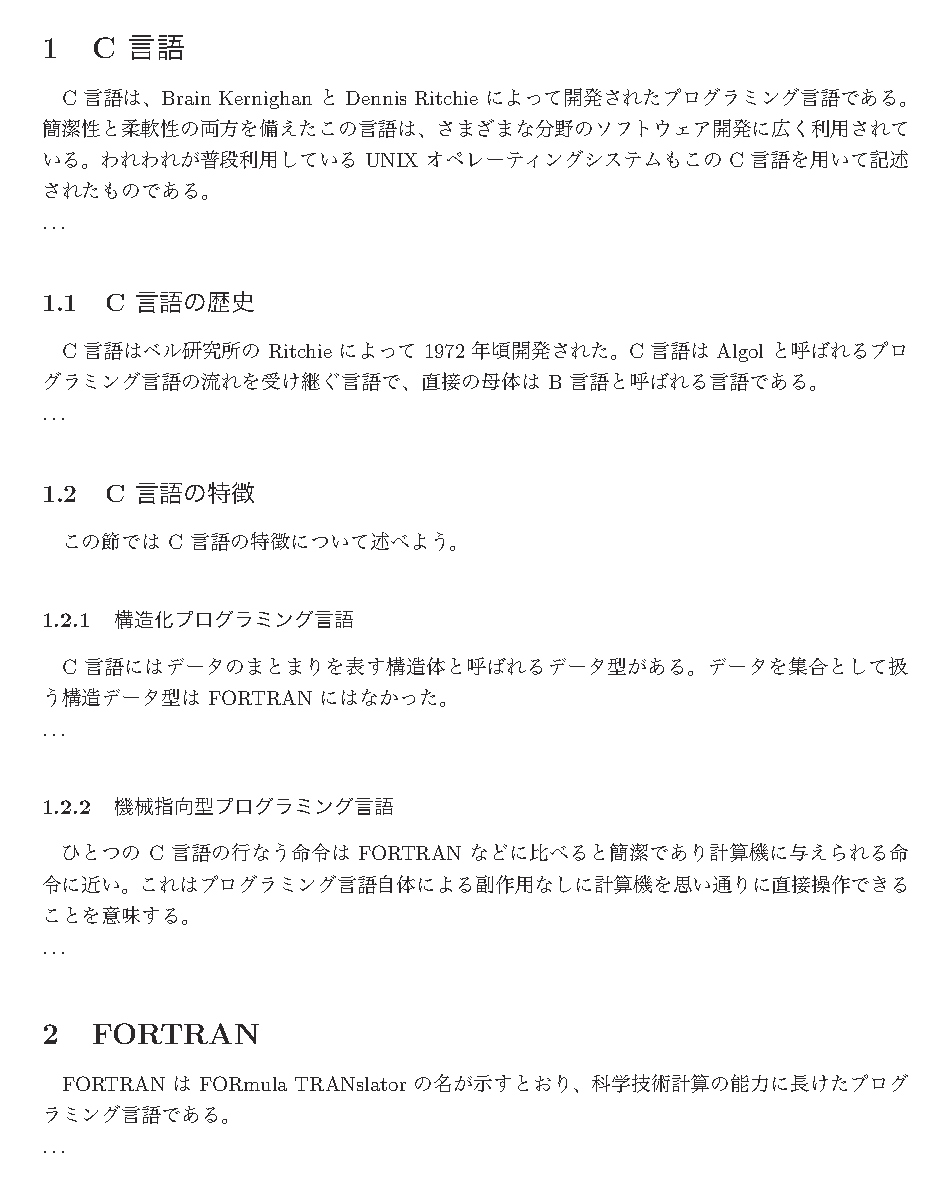
\includegraphics[bb=0 0 453 569, width=.9\textwidth]{section.pdf}
  \end{center}
\end{kekka}


\paragraph{この節のまとめ}

\begin{itemize}
\item 論文の表題は、\verb|\title{}| 、\verb|\author{}| 、\verb|\date{}| などで指定する。
\item 表題を出力するには、\verb|\maketile|を使う。
\item 章や節のタイトルを付けるには、\verb|\chapter{}|、\verb|\section{}|、 \verb|\subsection{}|、 \verb|\subsubsection{}| などを用いる。
\end{itemize}

\section{箇条書き}
\label{sec:latex:itemize}

論文の中では箇条書きを使うことは避けたほうがよいといわれている。特に、何かの処理の手順を説明するときは、箇条書きにするよりは言葉を使って説明するべきである。しかし、場合によっては箇条書きの方が説明が伝わりやすいこともある。単に項目を並列に並べたいときは箇条書きでもよいであろう。この節では箇条書きの方法を説明する。

箇条書きにしたいときは次のように書く。
\begin{reidai}
\begin{verbatim}
午後の紅茶(ミルクティー)の原材料名:
\begin{itemize}
  \item 牛乳
  \item 砂糖
  \item 加糖練乳
  \item 紅茶
  \item 香料
  \item 乳化剤
  \item ビタミン C
\end{itemize}
\end{verbatim}
\end{reidai} \noindent
このように、文章を\verb|\begin{itemize}|と\verb|\end{itemize}|とで囲むと、その領域は箇条書き環境になる。箇条書き環境の中では、\verb|\item|というコマンドを使うと新しい項目を始めることができる。
\begin{kekka}
  \def\labelitemisave{\labelitemi}
  \def\labelitemi{$\bullet$}
  午後の紅茶(ミルクティー)の原材料名:
  \begin{itemize}
  \item 牛乳
  \item 砂糖
  \item 加糖練乳
  \item 紅茶
  \item 香料
  \item 乳化剤
  \item ビタミン C
  \end{itemize}
  \def\labelitemi{\labelitemisave}
\end{kekka} \noindent
また、\texttt{itemize}の代わりに\texttt{enumerate}を使うと、各項目のラベルが1, 2, 3, $\cdots$のような番号となる。
\begin{reidai}
\begin{verbatim}
この講義の評価について該当するものに丸を付けて下さい。
\begin{enumerate}
\item 大変良かった。
\item まあまあ良かった。
\item 普通だった。
\item あまり良くなかった。
\item かなり良くなかった。
\end{enumerate}
\end{verbatim}
\end{reidai}
\vspace*{-1.5em}
\begin{kekka}
  この講義の評価について該当するものに丸を付けて下さい。
  \begin{enumerate}
  \item 大変良かった。
  \item まあまあ良かった。
  \item 普通だった。
  \item あまり良くなかった。
  \item かなり良くなかった。
  \end{enumerate}
\end{kekka}


\paragraph{この節のまとめ}

\begin{itemize}
\item \verb|\begin{itemize}| と \verb|\end{itemize}| で囲まれた部分は箇条書き環境になる。
\item \verb|\begin{enumerate}| と \verb|\end{enumerate}| で囲まれた部分は番号付き箇条書き環境になる。
\item 箇条書きの項目を始めるには\verb|\item|を使う。
\end{itemize}

\section{表の作成}
\label{sec:latex:table}

表を作成するには次に示す雛型を使えばよい。
\begin{reidai}
\begin{verbatim}
\begin{table}
  \begin{center}
    \caption{月刊誌の出版社と発売日}
    \begin{tabular}{|l|l|l|}
      \hline
      雑誌名 & 出版社 & 発売日 \\
      \hline \hline
      トランジスタ技術 & CQ出版 & 10 日 \\
      \hline
      UNIX Magazine & アスキー & 19 日 \\
      \hline
      SD ソフトウェアデザイン & 技術評論社 & 19 日 \\
      \hline
      アフタヌーン & 講談社 & 25 日 \\
      \hline
    \end{tabular}
  \end{center}
\end{table}
\end{verbatim}
\end{reidai}
\vspace*{-1.5em}
\begin{kekka}
  \begin{center}
    表1: 月刊誌の出版社と発売日 \\
    \begin{tabular}{|l|l|l|}
      \hline
      雑誌名 & 出版社 & 発売日 \\
      \hline \hline
      トランジスタ技術 & CQ出版 & 10 日 \\
      \hline
      UNIX Magazine & アスキー & 19 日 \\
      \hline
      SD ソフトウェアデザイン & 技術評論社 & 19 日 \\
      \hline
      アフタヌーン & 講談社 & 25 日 \\
      \hline
    \end{tabular}
  \end{center}
\end{kekka} \noindent
\verb|\hline| と書いたところには、横線が引かれる。\verb|\hline \hline|と2つ続けて書くと二重線になる。表の各行は、それぞれの要素の間を\texttt{\&}で区切り、最後に \texttt{\textbackslash \textbackslash} で改行して行が終わったことを\LaTeX に伝える。

この表は横の1行に3つの要素を持つ表である。各要素は表の1マスに左詰めで書かれている。このことは
\begin{quotation}
  \verb-\begin{tabular}{|l|l|l|}-
\end{quotation}
の\verb-{|l|l|l|}-によって表現されている。 \texttt{l} は左詰めを意味し、それを3つ並べることで、1行に3つの要素が入ることを表現しています。左詰めの代わりに中央揃えがよければ\texttt{c}を、右詰めがよければ\texttt{r}を指定する。

それぞれの\texttt{l}の両隣の縦棒は、要素と要素の間を縦線で区切って印刷してほしいということを\LaTeX に伝えている。この縦棒を取ってしまうと、要素間の縦線が引かれなくなる。

表の表題は
\begin{quotation}
  \verb|\caption{月刊誌の出版社と発売日}|
\end{quotation}
のように \verb|\caption| の後の \verb|{}| の中に書く。
最後にもう1つ例を挙げておこう。
\begin{reidai}
\begin{verbatim}
\begin{table}
  \begin{center}
    \caption{代表的な粒子の質量}
    \begin{tabular}{|c|r|}
      \hline
      粒子 & 質量 (MeV/$c^2$) \\
      \hline \hline
      $e ^ \pm$ & 0.5110 \\
      \hline
      $\mu ^ \pm$ & 105.7 \\
      \hline
      $\pi ^ \pm$ & 139.6 \\
      \hline
      $\pi ^ 0$ & 135.0 \\
      \hline
      $J/\psi$ & 3097 \\
      \hline
      $B ^ 0$ & 5279 \\
      \hline
    \end{tabular}
  \end{center}
\end{table}
\end{verbatim}
\end{reidai}
\vspace*{-1.5em}
\begin{kekka}
  \begin{center}
    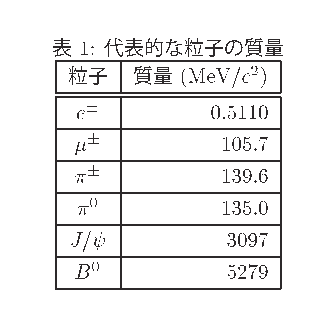
\includegraphics{table2.pdf}
  \end{center}
\end{kekka}

\section{数式}
\label{sec:latex:math}

数式は、例\ref{reidai:latex:ex}で見たとおり、
\begin{reidai}
\begin{verbatim}
\begin{equation}
%%% ここに数式を書きます %%%
\end{equation}
\end{verbatim}
\end{reidai} \noindent
というスタイルで記述する。\verb|\begin{equation}|と\verb|\end{equation}|とで囲まれた範囲では、数式環境の中のみで有効な様々なコマンドが使える。また、数式の番号は自動的に振られる。

結果\ref{kekka:ex}で見たとおり、\verb|\begin{equation}|と\verb|\end{equation}|とで囲まれた領域の数式は、改まった行の中央に表示される。しかし、場合によっては
\addtocounter{reidai}{1}
\begin{kekka}
  \label{kekka:math}
  $x$ の関数 $y = ax ^ 2 + bx + c$ のうち
  $a \ne 0$ であるものを $x$ の 2 次関数といいます。
\end{kekka} \noindent
\addtocounter{reidai}{-1}
のように文章中にインラインで数式を書きたいこともあるだろう。そういう場合は、文章中に\texttt{\$}と\texttt{\$}で囲った数式を書けばよい。結果\ref{kekka:math}を与えるソースは、以下のとおりである。
\begin{reidai}
\begin{verbatim}
$x$の関数$y = ax ^ 2 + bx + c$のうち
$a \ne 0$ であるものを$x$の2次関数といいます。
\end{verbatim}
\end{reidai} \noindent
以降の例題中ではスペースの都合上、2つ以上の数式を並べて書いてある場合があるが、、実際には1つずつ\verb|\begin{equation}|と\verb|\end{equation}|とで囲むか、\texttt{\$}と\texttt{\$}とで囲まなくてならない。

\subsection{添え字}
\label{sec:latex:index}

上付き添え字は\texttt{\^}で、上付き添え字は\texttt{\_}で表現する。
\begin{reidai}
\begin{verbatim}
y = a x ^ 2 + b x + c
S_n = a_1 + a_2 + a_3 + \cdots + a_n
\end{verbatim}
\end{reidai}
\vspace*{-1.5em}
\begin{kekka}
  \begin{equation*}
    y = a x ^ 2 + b x + c
  \end{equation*}
  \begin{equation*}
    S_n = a_1 + a_2 + a_3 + \cdots + a_n
  \end{equation*}
  \vspace{0pt}
\end{kekka} \noindent
2文字以上からなる項を添え字にしたいときは、\verb|{}|で添え字を囲む。
\begin{reidai}
\label{reidai:latex:2let_index}
\begin{verbatim}
Tr\,A = A_{11} + A_{22} + A_{33} + \cdots + A_{ii} + \cdots + A_{nn}
\end{verbatim}
\end{reidai}
\vspace*{-1.5em}
\begin{kekka}
  \begin{equation*}
    Tr\,A = A_{11} + A_{22} + A_{33} + \cdots + A_{ii} + \cdots + A_{nn}
  \end{equation*}
  \vspace{0pt}
\end{kekka} \noindent
添え字に限らず、\LaTeX の数式コマンドを2文字以上の項に作用させるときはかならず項を\verb|{}|で囲む必要がある。逆に1文字だけの項を\verb|{}|で囲んでも特に問題はない。なお、例\ref{reidai:latex:2let_index}の中で`\verb|\,|'というコマンドが使われているが、これはスペースの微調整をしたいときに使用する。

\subsection{分数}
\label{sec:latex:frac}

分数は\texttt{\textbackslash frac\{\textrm{分子}\}\{\textrm{分母}\}}の
ように表現する。
\begin{reidai}
\begin{verbatim}
1 + \frac{1}{2} = \frac{3}{2}
1 + \frac{1}{1+\frac{1}{2}} = \frac{5}{3}
\end{verbatim}
\end{reidai}
\vspace*{-1.5em}
\begin{kekka}
  \begin{equation*}
    1 + \frac{1}{2} = \frac{3}{2}
  \end{equation*}
  \begin{equation*}
    1 + \frac{1}{1+\frac{1}{2}} = \frac{5}{3}
  \end{equation*}
\end{kekka}

\subsection{関数}
\label{sec:latex:func}

数学環境では文字はすべて変数と見なされるため、\verb|cos x| という入力は$cos x$と斜体で印刷される。これではあたかも$c$、$o$、$s$、$x$の積のようである。数学関数は正しくは立体で表示されなくてはならない。立体で印刷するためには、\verb|\cos x|と入力する。このように数学関数の多くはバックスラッシュ(\texttt{\textbackslash})に関数名をつなげると表現できる。
\begin{reidai}
\begin{verbatim}
\frac{d}{dx} \sin x = \cos x
\end{verbatim}
\end{reidai}
\vspace*{-1.5em}
\begin{kekka}
  \begin{equation*}
    \frac{d}{dx} \sin x = \cos x
  \end{equation*}
\end{kekka}
\noindent
%ちなみに本当は、微分記号の $d$ も斜体ではなく立体で $\mathrm{d}$ と書くのが正統です。自然対数の底 $\mathrm{e}$、虚数単位 $\mathrm{i}$ など数学の分野で常識となっている量や記号には立体を、自分で定義した変数には斜体を使うことになっています。
表\ref{tab:func}に主な数学関数を示す。
\begin{table}[H]
  \begin{center}
    \caption{主な数学関数}
    \label{tab:func}
    \begin{tabular}{ccc}
      \verb|\cos| & \verb|\sin| & \verb|\tan| \\
      \verb|\cosh| & \verb|\sinh| & \verb|\tanh| \\
      \verb|\log| & \verb|\ln| & \verb|\exp| \\
      \verb|\lim| & & \\
    \end{tabular}
  \end{center}
\end{table}

\subsection{フォント}
\label{sec:latex:mathfont}

前節でも触れたが、\LaTeX は立体で印刷したい文字も斜体で印刷してしまうことがある。数式中でフォントを強制的に変更するときは前に説明した方法は使わない。数式中で立体の文字を印刷するには、\texttt{\textbackslash mathrm\{\textrm{文字}\}}と書く。
\begin{reidai}
\begin{verbatim}
\frac{\mathrm d}{\mathrm{d}x}\mathrm{e}^x = \mathrm{e}^x
\end{verbatim}
\end{reidai}
\noindent これにより、立体で表示されるべきところは正しく立体で印刷される。
\begin{kekka}
  \begin{equation*}
    \frac{\mathrm d}{\mathrm{d}x}\mathrm{e}^x = \mathrm{e}^x
  \end{equation*}
\end{kekka}

\subsection{積分・和・積}
\label{sec:latex:integration}

積分、和、積は以下のように表現する。
\begin{reidai}
\begin{verbatim}
\int _1 ^2 \frac{1}{x^2} \mathrm{d}x = \frac{1}{2}
\sum _{k=1} ^n k = \frac{n(n+1)}{2}
n! = \prod _{k=1} ^n k
\end{verbatim}
\end{reidai}
\vspace*{-1.5em}
\begin{kekka}
  \begin{equation*}
    \int _1 ^2 \frac{1}{x^2} \mathrm{d}x = \frac{1}{2}
  \end{equation*}
  \begin{equation*}
    \sum _{k=1} ^n k = \frac{n(n+1)}{2}
  \end{equation*}
  \begin{equation*}
    n! = \prod _{k=1} ^n k
  \end{equation*}
\end{kekka}

\subsection{根号・ベクトル・上線・チルダ・ハット・時間微分}
\label{sec:latex:root}

根号、ベクトル、上線の記号は以下のように表現する。
\begin{reidai}
\begin{verbatim}
\sqrt{x^2 + 2x + 1} = |x+1|
\vec{x} + \vec{y} = \vec{z}
\overrightarrow{OA} + \overrightarrow{AP} = \overrightarrow{OP}
\overline{x + \mathrm{i}y} = x - \mathrm{i}y
\end{verbatim}
\end{reidai}
\vspace*{-1.5em}
\begin{kekka}
  \begin{equation*}
    \sqrt{x^2 + 2x + 1} = |x+1|
  \end{equation*}
  \begin{equation*}
    \vec{x} + \vec{y} = \vec{z}
  \end{equation*}
  \begin{equation*}
    \overrightarrow{OA} + \overrightarrow{AP} = \overrightarrow{OP}
  \end{equation*}
  \begin{equation*}
    \overline{x + \mathrm{i}y} = x - \mathrm{i}y
  \end{equation*}
  \vspace{0pt}
\end{kekka}

同様にチルダ、ハット(演算子)、時間微分などは以下のように表現する。
\begin{reidai}
\begin{verbatim}
\tilde{x}
\hat{r}
\dot{x}
\end{verbatim}
\end{reidai}
\vspace*{-1.5em}
\begin{kekka}
  \begin{equation*}
    \tilde{x}
  \end{equation*}
  \begin{equation*}
    \hat{r}
  \end{equation*}
  \begin{equation*}
    \dot{x}
  \end{equation*}
  \vspace{0pt}
\end{kekka}

\subsection{ギリシャ文字}
\label{sec:latex:greek}

ギリシャ文字は文字を英語表記で綴り、前にバックスラッシュを付けると表示される。$\alpha$ は \verb|\alpha| と入力する。ギリシャ文字の大文字は、英語の綴りの最初の 1 文字を大文字にすると表示できる。 \verb|\Psi| と書けば $\Psi$ が印刷される。
\begin{table}[H]
  \begin{center}
    \caption{ギリシャ文字一覧}
    \label{tab:greek}
    \begin{tabular}{|lcc|lcc|lcc|}
      \hline
      コマンド & 小文字 & 大文字 & コマンド & 小文字 & 大文字 & コマンド & 小文字 & 大文字 \\
      \hline \hline
      \verb|\alpha| & $\alpha$ & -- & \verb|\iota| & $\iota$ & -- & \verb|\rho| & $\rho$ & -- \\
      \verb|\beta| & $\beta$ & -- & \verb|\kappa| & $\kappa$ & -- & \verb|\sigma| & $\sigma$ & $\Sigma$ \\
      \verb|\gamma| & $\gamma$ & $\Gamma$ & \verb|\lambda| & $\lambda$ & $\Lambda$ & \verb|\tau| & $\tau$ & -- \\
      \verb|\delta| & $\delta$ & $\Delta$ & \verb|\mu| & $\mu$ & -- & \verb|\upsilon| & $\upsilon$ & $\Upsilon$ \\
      \verb|\epsilon| & $\epsilon$ & -- & \verb|\nu| & $\nu$ & -- & \verb|\phi| & $\phi$ & $\Phi$ \\
      \verb|\zeta| & $\zeta$ & -- & \verb|\xi| & $\xi$ & $\Xi$ & \verb|\chi| & $\chi$ & -- \\
      \verb|\eta| & $\eta$ & -- & \verb|o| & $o$ & $O$ & \verb|\psi| & $\psi$ & $\Psi$ \\
      \verb|\theta| & $\theta$ & $\Theta$ & \verb|\pi| & $\pi$ & $\Pi$ & \verb|\omega| & $\omega$ & $\Omega$ \\
      \hline
    \end{tabular}
  \end{center}
\end{table} \noindent
-- となっている箇所は、通常のアルファベットの大文字で代用する。

\subsection{行列}
\label{sec:latex:matrix}

行列を書く方法は表の作成と似ている。
\begin{reidai}
\begin{verbatim}
\sigma_3 = (
\begin{array}{cc}
  1 & 0 \\
  0 & -1 \\
\end{array} )
\end{verbatim}
\end{reidai} \noindent
表のところで説明されている書き方のうち、\verb|\begin{tabular}| から\verb|\end{tabular}| までをまねして、 \texttt{tabular} を \texttt{array} に書き換える。行列の丸カッコは自動的には印刷されないので自分で書く\footnote{ちなみに、AMS\LaTeX では{\tt pmatrix}環境が用意されており、行列をより自然な形で記述できる。}。
\begin{kekka}
  \begin{equation*}
    \sigma_3 = (
    \begin{array}{cc}
      1 & 0 \\
      0 & -1 \\
    \end{array} )
  \end{equation*}
  \vspace{0pt}
\end{kekka} \noindent
しかし、これではカッコの大きさがあまり美しくない。カッコを括られている内容の高さに合わせて大きくするには、\verb|\left(| と \verb|\right)| を使う。
\begin{reidai}
\begin{verbatim}
\phi (x) = \sqrt{\frac{1}{2}} \left(
\begin{array}{c}
  0 \\
  v + h(x)
\end{array} \right)
\end{verbatim}
\end{reidai} \noindent
\vspace*{-1.5em}
\begin{kekka}
  \begin{equation}
    \phi (x) = \sqrt{\frac{1}{2}} \left(
      \begin{array}{c}
        0 \\
        v + h(x)
      \end{array} \right)
  \end{equation}
  \vspace{0pt}
\end{kekka} \noindent
\verb|\left(| と \verb|\right)| の組み合わせは、中に入るものが行列でなくても使える。また、丸カッコ以外にも使える。
\begin{reidai}
\begin{verbatim}
J_{\mu}^{NC}(\nu) =
\frac{1}{2}
\left[
\overline{u}_{\nu}\gamma_{\mu} \frac{1}{2} (1-\gamma^5)u_\nu
\right]
\end{verbatim}
\end{reidai}
\vspace*{-1.5em}
\begin{kekka}
  \begin{equation}
    J_{\mu}^{NC}(\nu) =
    \frac{1}{2}
    \left[
      \overline{u}_{\nu}\gamma_{\mu} \frac{1}{2} (1-\gamma^5)u_\nu
    \right]
  \end{equation}
  \vspace{0pt}
\end{kekka} \noindent
このようにカギカッコなどにも使える。

\subsection{特殊記号}
\label{sec:latex:symbol}

最後に \LaTeX で使える特殊記号を示しておく。
\begin{table}[H]
  \begin{center}
    \caption{主な特殊記号}
    \label{tab:symbol}
    \begin{tabular}{|lc|}
      \hline
      コマンド & 印刷結果 \\
      \hline \hline
      \verb|\ne| & $\ne$ \\
      \verb|\le| & $\le$ \\
      \verb|\ge| & $\ge$ \\
      \verb|\equiv| & $\equiv$ \\
      \verb|\pm| & $\pm$ \\
      \verb|\times| & $\times$ \\
      \verb|\infty| & $\infty$ \\
      \verb|\bullet| & $\bullet$ \\
      \verb|\prime| & $\prime$ \\
      \verb|\dagger| & $\dagger$ \\
      \verb|\partial| & $\partial$ \\
      \verb|\to| & $\to$ \\
      \verb|\nabla| & $\nabla$ \\
      \verb|\triangle| & $\triangle$ \\
      \hline
    \end{tabular}
  \end{center}
\end{table}

\paragraph{この節のまとめ}

\begin{itemize}
\item 数式を書くには、\verb|\begin{equation}|と\verb|\end{equation}|で囲む。
\item 文章中で数式を書くには \texttt{\$} と \texttt{\$} で囲む。
\item 添え字、分数、関数、積分記号などについては、それぞれにコマンドが用意されている。
\end{itemize}

\section{図の貼り込み}
\label{sec:latex:picture}

\LaTeX では、{\tt gnuplot}などで生成した(\ref{sec:unix:gnuplot})節)図のファイル(ポストスクリプト、PDFなど)を文章中に貼り込むことが可能である。

%% \subsection{EPS ファイルの作成}
%% \label{sec:latex:make_eps}

%% 最近では Tgif や xfig などさまざまな描画ソフトウェアが EPS 形式の図を
%% 出力してくれます。ここでは、描画ツールの 1 つである GNUPLOT を使って
%% EPS 形式のファイルを作る説明をします。 GNUPLOT はグラフを表示する機能が
%% 秀でたソフトウェアです。

%% まずは GNUPLOT を起動し、画面に図を表示させましょう。
%% \begin{commandline}
%% \begin{verbatim}
%% example% gnuplot
%% gnuplot> plot x*x
%% \end{verbatim}
%% \end{commandline}
%% これで $y = x^2$ のグラフが表示されました。
%% \begin{commandline}
%% \verb|gnuplot> set term postscript|\\
%% \verb|gnuplot> set output |\textrm{"\textit{filename}"}\\
%% \verb|gnuplot> replot|
%% \end{commandline}
%% ここまでの操作で $y = x^2$ のグラフの絵が \textit{filename} という
%% 名前のファイルに保存されます。 \textit{filename} は自分で
%% 適当なものを決めます。ただし拡張子は \texttt{.ps} にしておきましょう。
%% 以下では \textit{filename} は \texttt{test.ps} という名前にしたことにします。
%% もう GNUPLOT は使わないので終了します。
%% \begin{commandline}
%% \begin{verbatim}
%% gnuplot> quit
%% example%
%% \end{verbatim}
%% \end{commandline}
%% さて \texttt{test.ps} というファイルですがまだ EPS 形式にはなっておらず、
%% PS という形式になっています。このファイルを EPS 形式にするには
%% \texttt{ps2epsi} というコマンドを使います。
%% \begin{commandline}
%% \begin{verbatim}
%% example% ps2epsi test.ps
%% \end{verbatim}
%% \end{commandline}
%% これで \texttt{test.epsi} というファイルができます。
%% \texttt{test.epsi} は EPS 形式になっていますので、これは \LaTeX の文章中に
%% 貼り込むことができます。次の節では実際に図を貼り込む方法について
%% 説明しましょう。

\subsection{EPS ファイルの貼り込み}
\label{sec:latex:include_eps}

図を貼り込むには以下の雛型を用いる。
\begin{reidai}
\begin{verbatim}
\begin{figure}
  \begin{center}
    \includegraphics[width=8cm,clip]{test.eps}
    \caption{$y = x^2$ のグラフ}
  \end{center}
\end{figure}
\end{verbatim}
\end{reidai}
\vspace*{-1.5em}
\begin{kekka}
  \begin{center}
    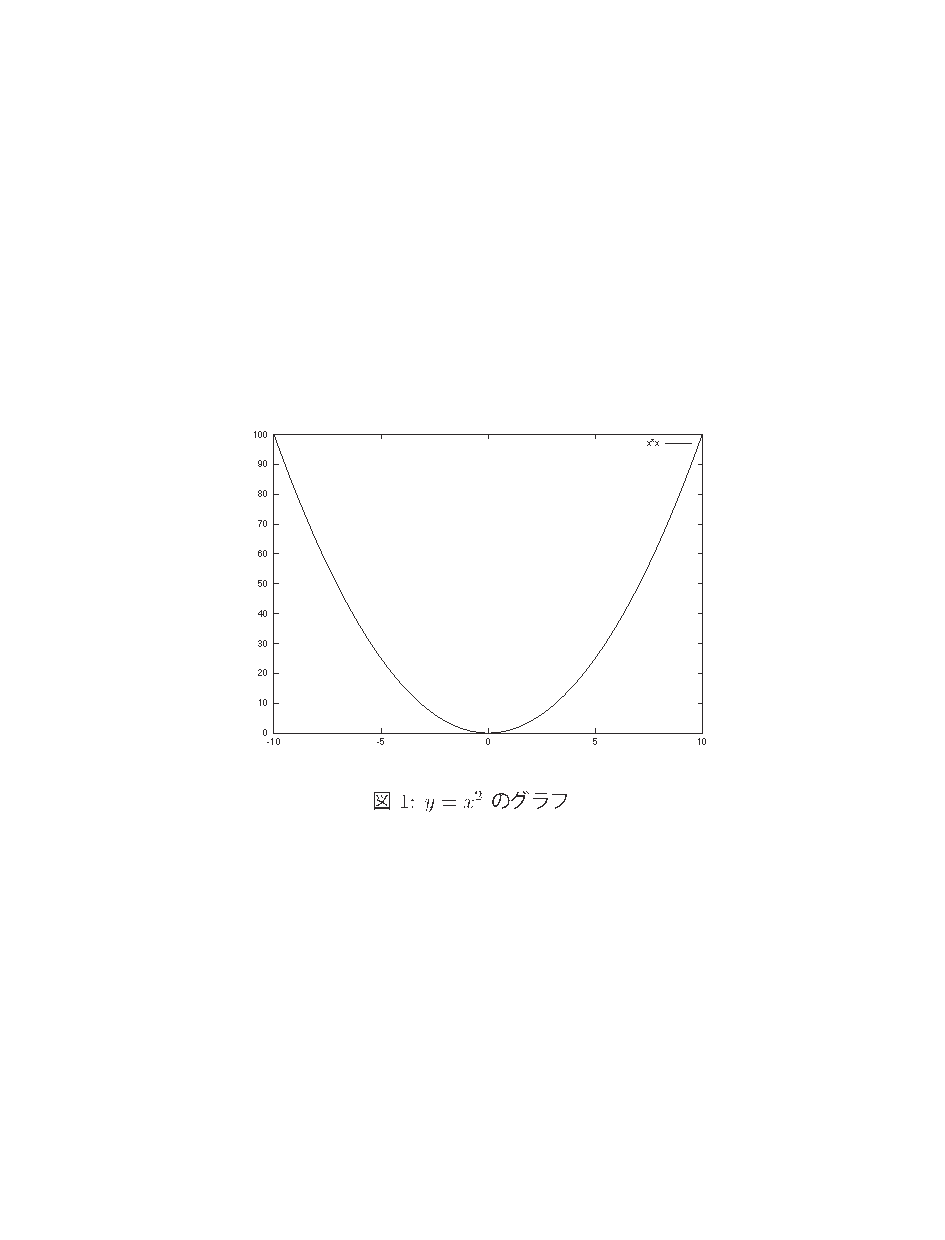
\includegraphics{figure.pdf}
  \end{center}
\end{kekka} \noindent
注意すべきところは
\begin{quotation}
  \verb|\includegraphics[width=8cm,clip]{test.eps}|
\end{quotation}
という部分である。ファイル名は{\tt \{\}}の中で指定する。また \texttt{width=8cm} という記述により図の横幅を指定している。図の表題も表のときと同じく \verb|\caption| コマンドを使う。

\LaTeX は図表を自動的に適切な位置に配置してくれるが、\verb|begin{figure}| の後に \texttt{[h]} を付けると、その場に配置することができる。それでもうまくいかない場合には、\texttt{here.sty}を使い、\textbf{例題 \ref{reidai:latex:here}}のように\verb|begin{figure}| の後に \texttt{[H]} を付けることにより、強制的に指定の位置に配置することも出来る。
\begin{reidai}
\label{reidai:latex:here}
\begin{verbatim}
\documentclass{jarticle}
\usepackage{graphicx}
\usepackage{here}

\begin{document}
\begin{figure}[H]
  \begin{center}
    \includegraphics{test.epsi}
    \caption{$y = x^2$ のグラフ}
  \end{center}
\end{figure}
\end{document}
\end{verbatim}
\end{reidai}

\subsection{図の回転}
\label{sec:latex:rotate_eps}

貼り込みたいファイル中の図が 90 度回転してしまっていることがある。\LaTeX では図を貼り込むときに回転させることができる。
\begin{reidai}
\begin{verbatim}
  \rotatebox{-90}{
    \includegraphics[width=8cm,clip]{test.eps}
  }
\end{verbatim}
\end{reidai} \noindent
このように、 \verb|\rotatebox{-90}| を使うことにより、図を -90 度回転させることができる。


\paragraph{この節のまとめ}

\begin{itemize}
\item \LaTeX の文章には、ポストスクリプトあるいはPDF形式の図を貼り込める。
\item 実際に図を貼り込むには雛型を使う。
\item 貼り込む図を回転させるには \verb|\rotatebox{角度}{}| を使う。
\end{itemize}

\section{参照と参考文献}
\label{sec:latex:ref_and_bib}

\subsection{参照}
\label{sec:latex:reference}

\LaTeX には、数式や表、図に付いた番号を簡単に参照する機能が用意されている。まずは具体例から見ていこう。
\begin{reidai}
\label{reidai:latex:noref}
\begin{verbatim}
媒質中を物質が通過するとき、チェレンコフ光が発生するための条件は
\begin{equation}
n > \frac{1}{\beta} = \sqrt{1+\left(\frac{m}{p}\right)^{2}}
\end{equation}
である。ただし式(1) において、
$n$ は媒質の屈折率、$m$ は物質の質量、$p$ は物質の運動量である。
\end{verbatim}
\end{reidai} \noindent
この清書結果は次のようになる。
\begin{kekka}
  媒質中を物質が通過するとき、チェレンコフ光が発生するための条件は
  \begin{equation}
    n > \frac{1}{\beta} = \sqrt{1+\left(\frac{m}{p}\right)^{2}}
  \end{equation}
  である。ただし式(1) において、
  $n$ は媒質の屈折率、$m$ は物質の質量、$p$ は物質の運動量である。\\
\end{kekka} \noindent
\textbf{例題 \ref{reidai:latex:noref}} ではチェレンコフ光の発生条件の式を
本文中に「式(1)」とハードコーティングしている。

さて、 \textbf{例題 \ref{reidai:latex:noref}} の式の前に別の式を挿入することになったとする。すると、式の番号はすべて 1 つずつ繰り下がるので、文章中で「式(1)」と書いているところをすべて「式(2)」に書き直さなければならない。このような番号の付け替えを手で行うのはとても大変であるし、間違いが起こりやすい。

こういった手間を省くために、 \LaTeX には数式や表・図に名前を
割り当てる機能が用意されている。
\begin{reidai}
\label{reidai:latex:ref}
\begin{verbatim}
媒質中を物質が通過するとき、チェレンコフ光が発生するための条件は
\begin{equation}
n > \frac{1}{\beta} = \sqrt{1+\left(\frac{m}{p}\right)^{2}} \label{cherenkov}
\end{equation}
である。ただし式(\ref{cherenkov}) において、
$n$ は媒質の屈折率、$m$ は物質の質量、$p$ は物質の運動量である。
\end{verbatim}
\end{reidai} \noindent
\textbf{例題 \ref{reidai:latex:ref}} は\textbf{例題 \ref{reidai:latex:noref}} と
同じ清書結果を与える。

数学環境中で \verb|\label| を使うとその数式に名前が付けられる。付ける名前は \verb|\label| の後の \verb|\{\}| の中に記述する。\textbf{例題 \ref{reidai:latex:ref}} では \texttt{cherenkov} という名前が付けられている。

さて、名前の付けられた数式をその名前で参照すると、その箇所が数式の番号に展開される。参照は \verb|\ref| コマンドを使う。\textbf{例題 \ref{reidai:latex:ref}} では \verb|\ref{cherenkov}| として参照している。\verb|\label{cherenkov}| によって名前付けした数式の番号は 1 だったので、 \verb|\ref{cherenkov}| の参照によってこれが 1 に展開されることになる。

以下に参照の例を挙げておく。
\begin{reidai}
\begin{verbatim}
本年度の遠足について、以下のとおり決定いたしましたのでお知らせします。
\begin{table}
  \begin{center}
    \caption{遠足の目的地(学年別)}
    \label{destination}
    \begin{tabular}{|l|l|}
      \hline
      学年 & 目的地 \\
      \hline \hline
      4 年生 & 近くにある公園 \\
      \hline
      5 年生 & 遠くにある公園 \\
      \hline
      6 年生 & かなり遠くにある公園 \\
      \hline
    \end{tabular}
  \end{center}
\end{table}
表 \ref{destination} をよく読んで自分の目的地をきちんと確認し、
遠足の目的地に相応しい準備をするように心がけてください。
\\
なお、おやつの持参は
\begin{equation}
\sum^{全おやつ} 各おやつの購入金額 \le 500 円 \label{oyatu}
\end{equation}
を条件とします。
ただし、バナナは 式(\ref{oyatu})にかかわらず好きなだけ持参して差しつかえありません。
\end{verbatim}
\end{reidai}
\vspace*{-1.5em}
\begin{kekka}
  \begin{center}
    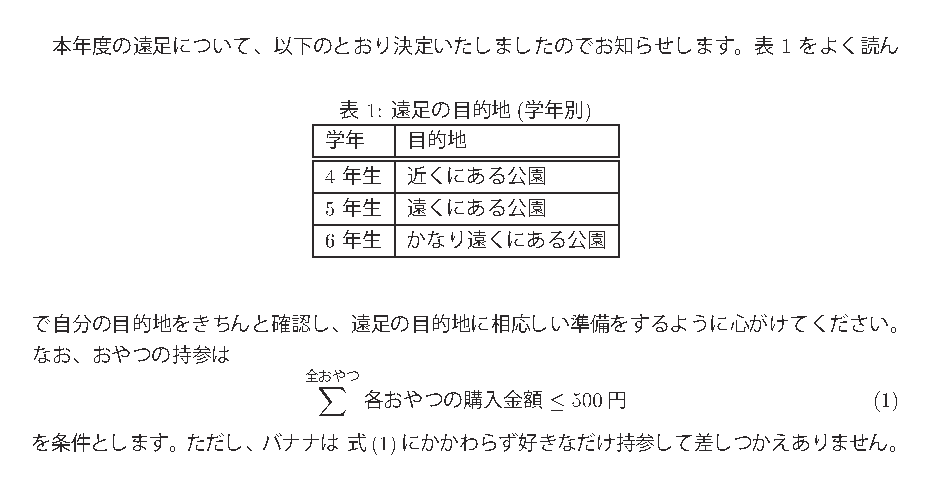
\includegraphics[bb=0 0 453 231,width=.9\textwidth]{ref.pdf}
  \end{center}
\end{kekka}


\subsection{参考文献}
\label{sec:latex:bibliography}

論文やレポートでは、通常、末尾に参考文献リストを付ける。
参考文献の番号も数式などと同じように自動的に振ることができる。
\begin{reidai}
\begin{verbatim}
第 1 象限内の複素数 $z$ について、
\begin{equation}
w(z) \equiv \mathrm{e}^{-z^2}\mathrm{erfc}(z)
\end{equation}
を近似的に計算するアルゴリズムが存在し \cite{wofz}、
その計算誤差は $10 ^ {-10}$ 以下である。
\\
このアルゴリズムは、 BELLE 実験 \cite{BELLE} で使用するプログラムの内部で利用されている。

...

\begin{thebibliography}{99}
\bibitem{wofz}
  Walter Gautschi, Comm ACM. \textbf{12} 635, (1969) 
\bibitem{BELLE}
  The BELLE Collaboration, KEK Report 95-1 (1995)
\end{thebibliography}
\end{verbatim}
\end{reidai}
\setcounter{equation}{0}
\vspace*{-1.5em}
\begin{kekka}
  \hspace*{0.3cm}第 1 象限内の複素数 $z$ について、
  \begin{equation}
    w(z) \equiv \mathrm{e}^{-z^2}\mathrm{erfc}(z)
  \end{equation}
  を近似的に計算するアルゴリズムが存在し[1]、
  その計算誤差は $10 ^ {-10}$ 以下である。
  \\
  このアルゴリズムは、 BELLE 実験[2]で使用するプログラムの
  内部で利用されている。

  \dots

  \noindent {\bf \Large 参考文献} \\

  \noindent [1] Walter Gautschi, Comm ACM. \textbf{12} 635, (1969)

  \noindent [2] The BELLE Collaboration, KEK Report 95-1 (1995)
\end{kekka} \noindent
文章中に書く \verb|\cite| では引用する論文の名前を指定する。論文の名前は自分が覚えやすいものであれば何でも構わないが、\verb|\bibitem| によって名前が定義されている必要がある。\verb|\bibitem| は \verb|\begin{thebibliography}| と \verb|\end{thebibliography}| とで囲まれた領域に書く。この領域は清書すると参考文献の章となる。
%参考文献はふつうは論文の最後の方に書きますので、
%\verb|\begin{thebibliography}| から \verb|\end{thebibliography}| までの
%領域も最後に書くのが自然でしょう。
\verb|\bibitem| に続く {\tt \{\}} の中には自分で決めた論文名を書く。この名前が \verb|\cite| によって参照されることになる。その後あとには、その論文の著者名や収録されている雑誌名などを書く。ここに書いたことは、参考文献の章が清書されるときにそのまま印刷される。

\verb|\cite| と \verb|\ref| を、 \verb|\bibitem| と \verb|\label| を
それぞれ対応付けて覚えておこう。


\subsection{コンパイル}
\label{sec:latex:compile}

参照を含むソースファイルを \LaTeX で処理するときは、\texttt{platex} コマンドを何回か実行する必要がある。これは、 \texttt{platex} が参照関係を解決することが、 1 回のコマンド実行だけではできないからである。参照が解決できていない状態では、展開されるべき参照の部分が ?? と表示される。\texttt{platex} の実行を何回か繰り返し、 ?? になっている参照がなくなったことを確認すること。

\paragraph{この節のまとめ}

\begin{itemize}
\item 数式や表、図には \verb|\label{名前}| で名前を付けられる。
\item 数式などに付けられた番号は、 \verb|\label{名前}| で付けた名前を手掛かりにして \verb|\ref{名前}| と書くことで参照できる。
\item 参考文献は \verb|\cite{論文名}| のようにして参照する。
\item 参考にした論文は、 \verb|\begin{thebibliography}| から
    \verb|\end{thebibliography}| までの領域に書く。
\item 論文は \verb|\bibitem{論文名}| 著者、雑誌名 \dots のように列挙する。
\item 参照を含むソースファイルに対しては、何回か \texttt{platex} コマンドを
  実行する必要がある。
\end{itemize}
